\documentclass[UTF8]{ctexart}
\usepackage{mathtools,wallpaper}

\usepackage{t1enc}
\usepackage{pagecolor}
\usepackage{geometry}
\usepackage{diagbox}
\usepackage{graphicx}
\usepackage{wrapfig}
\usepackage{amssymb}

\geometry{left=2cm,right=2cm}

\begin{document}

\CTEXsetup[format={\Large\bfseries}]{section}
\title{实验报告}  
\author{徐亦昶 PB20000156}
\maketitle
\section{实验题目}整流滤波和直流电源特性实验
\section{实验目的}
\begin{enumerate}
    \item 了解交流信号的几个参数
    \item 学习整流滤波电路的基本工作原理及制作一台直流电源
    \item 掌握直流电源特性的测量方法
    \item 了解负载对电源输出特性的影响
    \item 掌握非线性内阻电源开路电压和短路电流的测量方法
\end{enumerate}
\section{实验原理}
\subsection{纹波系数}
直流电源在直流稳定量上的交流分量称为纹波,一般可以用交流成分的有效值来表示纹波绝对强度的大小。纹波系数是指负载上交流电压的有效值与直流电压之比,
可用公式表示如下:
\newline
纹波系数$K_u=\frac{V_\sim}{V_-}\times 100\%$
\newline
其中$V_\sim$为交流电压有效值,$V_-$为直流电压。
\subsection{电源开路电压和短路电流}
由于电压表的内阻有限,而电流表内阻也不可能为零,而且电源短路的时候容易烧毁电源,因此不能直接用电压表或电流表测量电源的开路电压和短路电流。
对于干电池之类的电源,因为具有非线性内阻,因此也不适用 U-I 曲线外推法进行测量。
可以采用等效电路或补偿法来进行测量,电路图如下:
\begin{figure}[h]
    \centering
    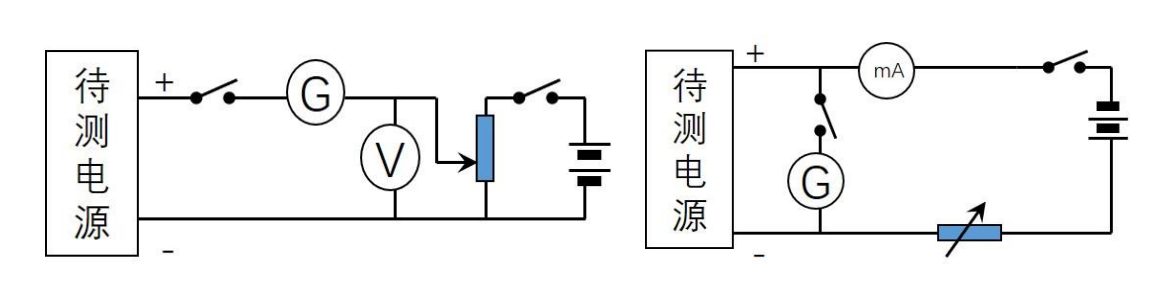
\includegraphics[scale=0.7]{电路图.PNG}
    \caption{等效电路法测量开路电压和短路电流电路图}
\end{figure}
对于左图,调节变阻器使G的示数为0,此时V的示数即为开路电压;对于右图,调节变阻器使G的示数为0,此时A的示数即为短路电流。
\section{实验内容}
\subsection{整流、滤波实验}
\begin{enumerate}
    \item 整流实验:采用如图4所示电路,用示波器观测信号源功率输出端输出纯正弦函数波形(无直流偏置),并把此正弦波峰峰值固定在 10 V,频率为 400Hz,在面包板上
    把元件分别连成半波、全波整流电路,把信号源接入到电路的输入端;用示波器分别观 察初始信号、半波、全波整流的输出端信号
    $u_0$,分别画出$u_0$ 的波形。
    \item 滤波实验:采用如图2所示电路,用示波器观察并画出输出端波形, 同时用万
    用表测量负载上的直流和交流电压,计算纹波系数;按图3连接π型RC电路进行滤波,用
    示波器观察并画出输出端波形,同时用万用表测量负载上的直流和交流电压,计算纹波系数。
\end{enumerate}
\subsection{不同负载下纹波系数的测量}
\begin{enumerate}
    \item 测量负载功率曲线:信号源选 500Hz 频率Vp-p=10V,正弦交流信号;电容选 1μF,在面包板上连接 π 型全波整流滤波电路,负载$R_L$连接电阻箱。
    在 20~2000Ω 范围内测量该电源的负载功率曲线。
    \item 测量纹波系数曲线:同上述电路,负载电阻在 20~2000Ω 范围内变化,测量输出端的直流、交流电压,并计算不同负载时该电源的纹波系数 Ku。绘制 Ku随负载 RL的变化曲线。
    \item 电容对纹波系数的影响:改用单个 10 μF 电容,连接全波整流滤波电路,重复上述内容,根据结果分析优劣。
\end{enumerate}
\begin{figure}[h!]
    \centering
    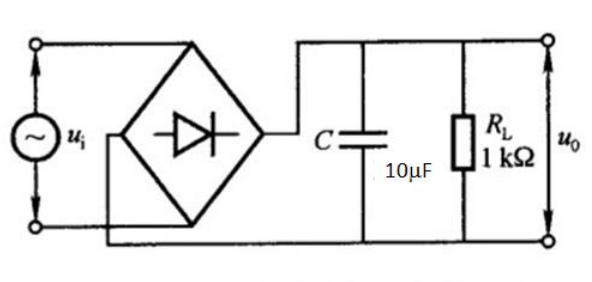
\includegraphics[scale=0.7]{全波整流电容滤波器.PNG}
    \caption{全波整流电容滤波器}
\end{figure}
\begin{figure}[h!]
    \centering
    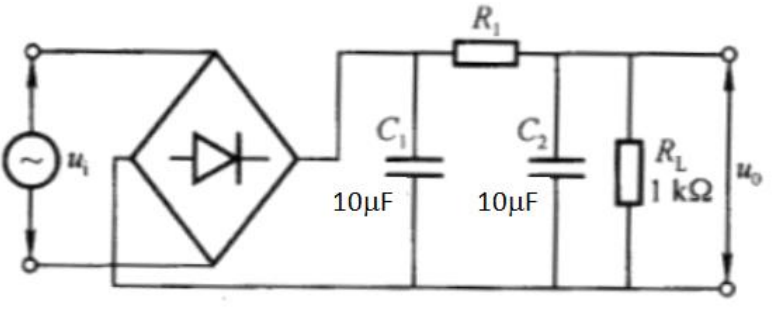
\includegraphics[scale=0.7]{pi型RC滤波电路.PNG}
    \caption{$\pi$型RC滤波电路}
\end{figure}
\begin{figure}[h!]
    \centering
    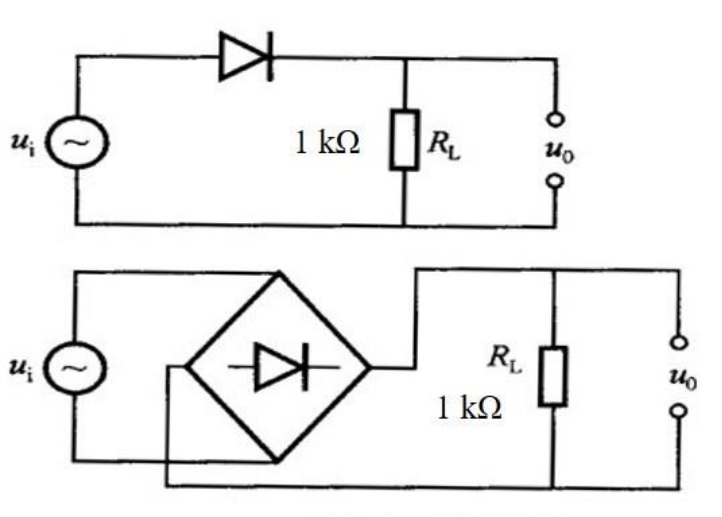
\includegraphics[scale=0.7]{半波和全波整流电路.PNG}
    \caption{半波和全波整流电路}
\end{figure}
\newpage
\section{数据记录}
\begin{table*}[htbp]
    \centering
    \fontsize{8}{10}\selectfont
    \caption{滤波实验}
    \scalebox{1.15}{
    \begin{tabular}{|c|c|c|}
    \hline
     &直流电压(V) & 交流电压(V) \\
    \hline
     $\pi$型 & 1.4869 &0.0650 \\
     \hline
     单电容 & 4.122 & 0.0047 \\
     \hline
    \end{tabular}}
\end{table*}
\begin{table*}[htbp]
    \centering
    \fontsize{8}{10}\selectfont
    \caption{负载功率测量}
    \scalebox{1.15}{
    \begin{tabular}{|c|c|c|c|c|c|c|c|c|c|c|c|}
    \hline
    R($\Omega$)&20&200&400&600&800&1000&1200&1400&1600&1800&2000 \\
    \hline
     U(V)&0.0373&0.3392&0.6197&0.8540&1.0524&1.2231&1.3715&1.5019&1.6176&1.7209&1.8140\\
     \hline
     P(mW)&0.0696&0.5753& 0.9600& 1.2155&1.3844& 1.4960& 1.5675& 1.6112&1.6354& 1.6453& 1.6453\\
     \hline
    \end{tabular}}
\end{table*}
\begin{table*}[htbp]
    \centering
    \fontsize{8}{10}\selectfont
    \caption{纹波系数测量}
    \scalebox{1.15}{
    \begin{tabular}{|c|c|c|c|c|c|c|c|c|c|c|c|}
    \hline
    R($\Omega$)&20&200&400&600&800&1000&1200&1400&1600&1800&2000 \\
    \hline
     $V_-(V)$&0.0374&0.3390&0.6197&0.8542&1.0523&1.2231&1.3713&1.5021&1.6177&1.7209&1.8143 \\
     \hline
     $V_\sim(V)$&0.0157&0.1053&0.1366&0.1428&0.1409&0.1361&0.1304&0.1247&0.1192&0.1139&0.1090 \\
     \hline
     $K_u$&0.4198&0.3106&0.2204&0.1672&0.1339&0.1113&0.0951&0.0830&0.0737&0.0662&0.0601 \\
     \hline
    \end{tabular}}
\end{table*}
\begin{table*}[htbp]
    \centering
    \fontsize{8}{10}\selectfont
    \caption{电容对纹波系数的影响}
    \scalebox{1.15}{
    \begin{tabular}{|c|c|c|c|c|c|c|c|c|c|c|c|}
    \hline
    R($\Omega$)&20&200&400&600&800&1000&1200&1400&1600&1800&2000 \\
    \hline
     $V_-(V)$&0.0049&0.4280&0.7631&1.0285&1.2457&1.4275&1.5821&1.7150&1.8313&1.9339&2.018 \\
     \hline
     $V_\sim(V)$&1.67&3.04&2.78&2.56&2.41&0.00&0.00&0.00&0.00&0.00&0.00 \\
     \hline
     $K_u$&340.816&7.103&3.643&2.489&1.935&0.000&0.000&0.000&0.000&0.000&0.000 \\
     \hline
    \end{tabular}}
\end{table*}
\section{数据计算}
滤波实验中,$\pi$型和单电容滤波器的波纹系数分别为4.37\%,0.11\%。
使用包含两个隐含层(维数为$5\times10$)的人工神经网络进行拟合,得到负载功率曲线如图:
\begin{figure}[h!]
    \centering
    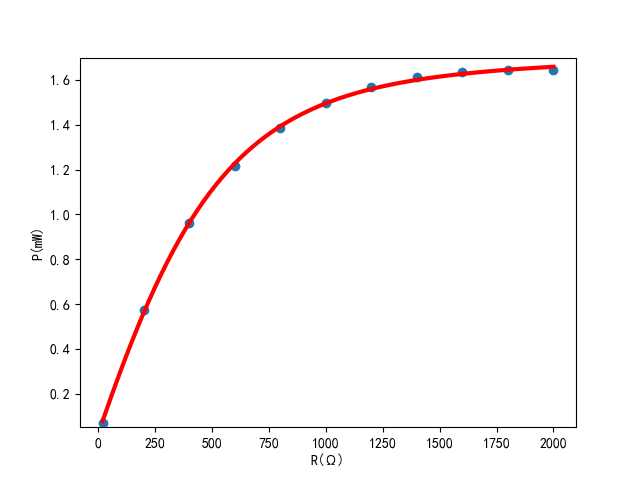
\includegraphics[scale=0.7]{负载功率曲线.png}
    \caption{负载功率曲线}
\end{figure}
\newline
$R=2000\Omega$时负载功率最大(负载功率随R增大而减小)。
\newline
拟合的纹波系数曲线如图:
\begin{figure}[h!]
    \centering
    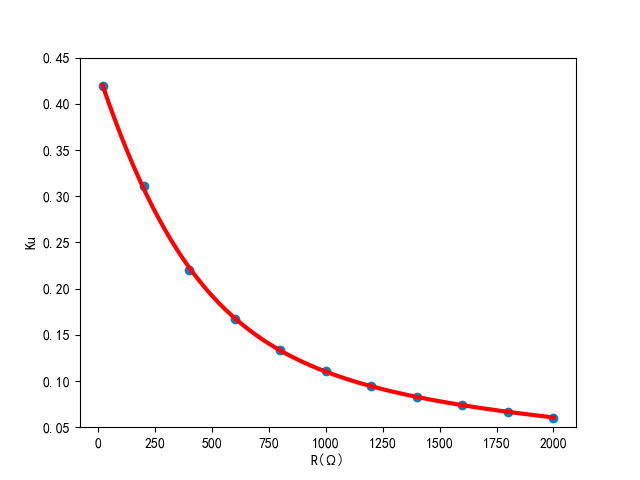
\includegraphics[scale=0.7]{纹波系数曲线.png}
    \caption{纹波系数曲线}
\end{figure}
\newline
换$10\mu F$的电容,测试电容对纹波系数的影响:
\begin{figure}[h!]
    \centering
    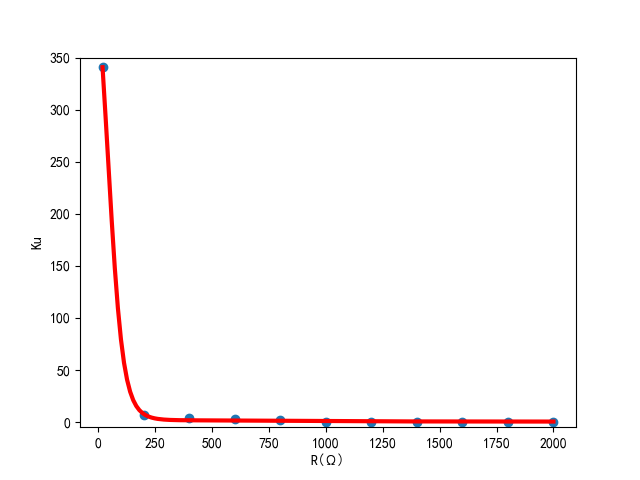
\includegraphics[scale=0.7]{电容对纹波系数的影响.png}
    \caption{$10\mu F$电容下纹波系数曲线}
\end{figure}
\newline
显然此时滤波性能优于之前选$1\mu F$电容时的滤波性能。
\newpage
\section{思考}
\begin{enumerate}
    \item 大电容滤出的波波纹系数更小,更接近直流电,但是直流电压有效值较小;小电容滤出的波波纹系数较大,但直流电压有效值较大。
    \item 整流、滤波的主要目的是将直流电中的交流成分去掉将纯净的直流供给负载
    \item 滤波电路中电容不是越大越好,大电容会降低滤出的波的直流电压有效值。
\end{enumerate}
\end{document}